\documentclass[koma,a4paper]{article}
\usepackage[T1]{fontenc}
\usepackage[danish]{babel}
\usepackage{fixltx2e}
\usepackage{graphicx}
\usepackage{float}
\usepackage{amsmath}
\usepackage{amssymb}
\usepackage[hidelinks]{hyperref}
\usepackage{amsthm}
\usepackage{tikz}
\usepackage{todonotes}
\usepackage{booktabs}
\usepackage{subcaption}
\usepackage{color}
\usepackage{lmodern}
\graphicspath{{graphics/}}
\usetikzlibrary{trees}

\newcommand*\circled[1]{\tikz[baseline=(char.base)]{\node[shape=circle,draw,inner sep=2pt] (char) {#1};}} % circles around numbers

\title{AALG Self Study 3}
\author{Andreas Petersen\\
Mads E. Kalør\\
Søren B. Ranneries\\
Room 1.1.34}
\begin{document}
\maketitle

\pagebreak

\section{Exercise 1}

\subsection{A}
Figure \ref{fig:vertices_capacity} shows how to convert a vertex with capacity to a regular flow network. The number of edges in a network with vertex capacities is $2|V|$ in a regular flow network, and the number of edges is $|V|+|E|$.

\begin{figure}
  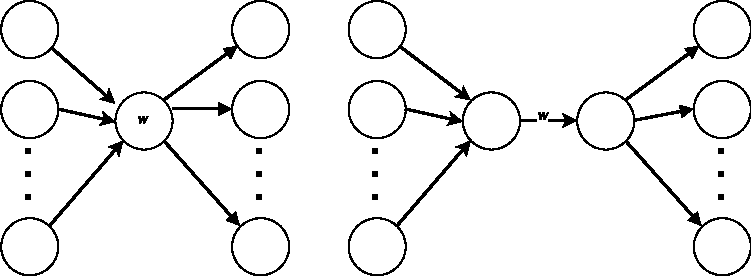
\includegraphics{weighted_vertices}
  \caption{Vertices with capacity}
  \label{fig:vertices_capacity}
\end{figure}

\end{document}
